\section{Generating PFunc's interface}
\label{sec:generate}

\begin{figure}[t]
\centering
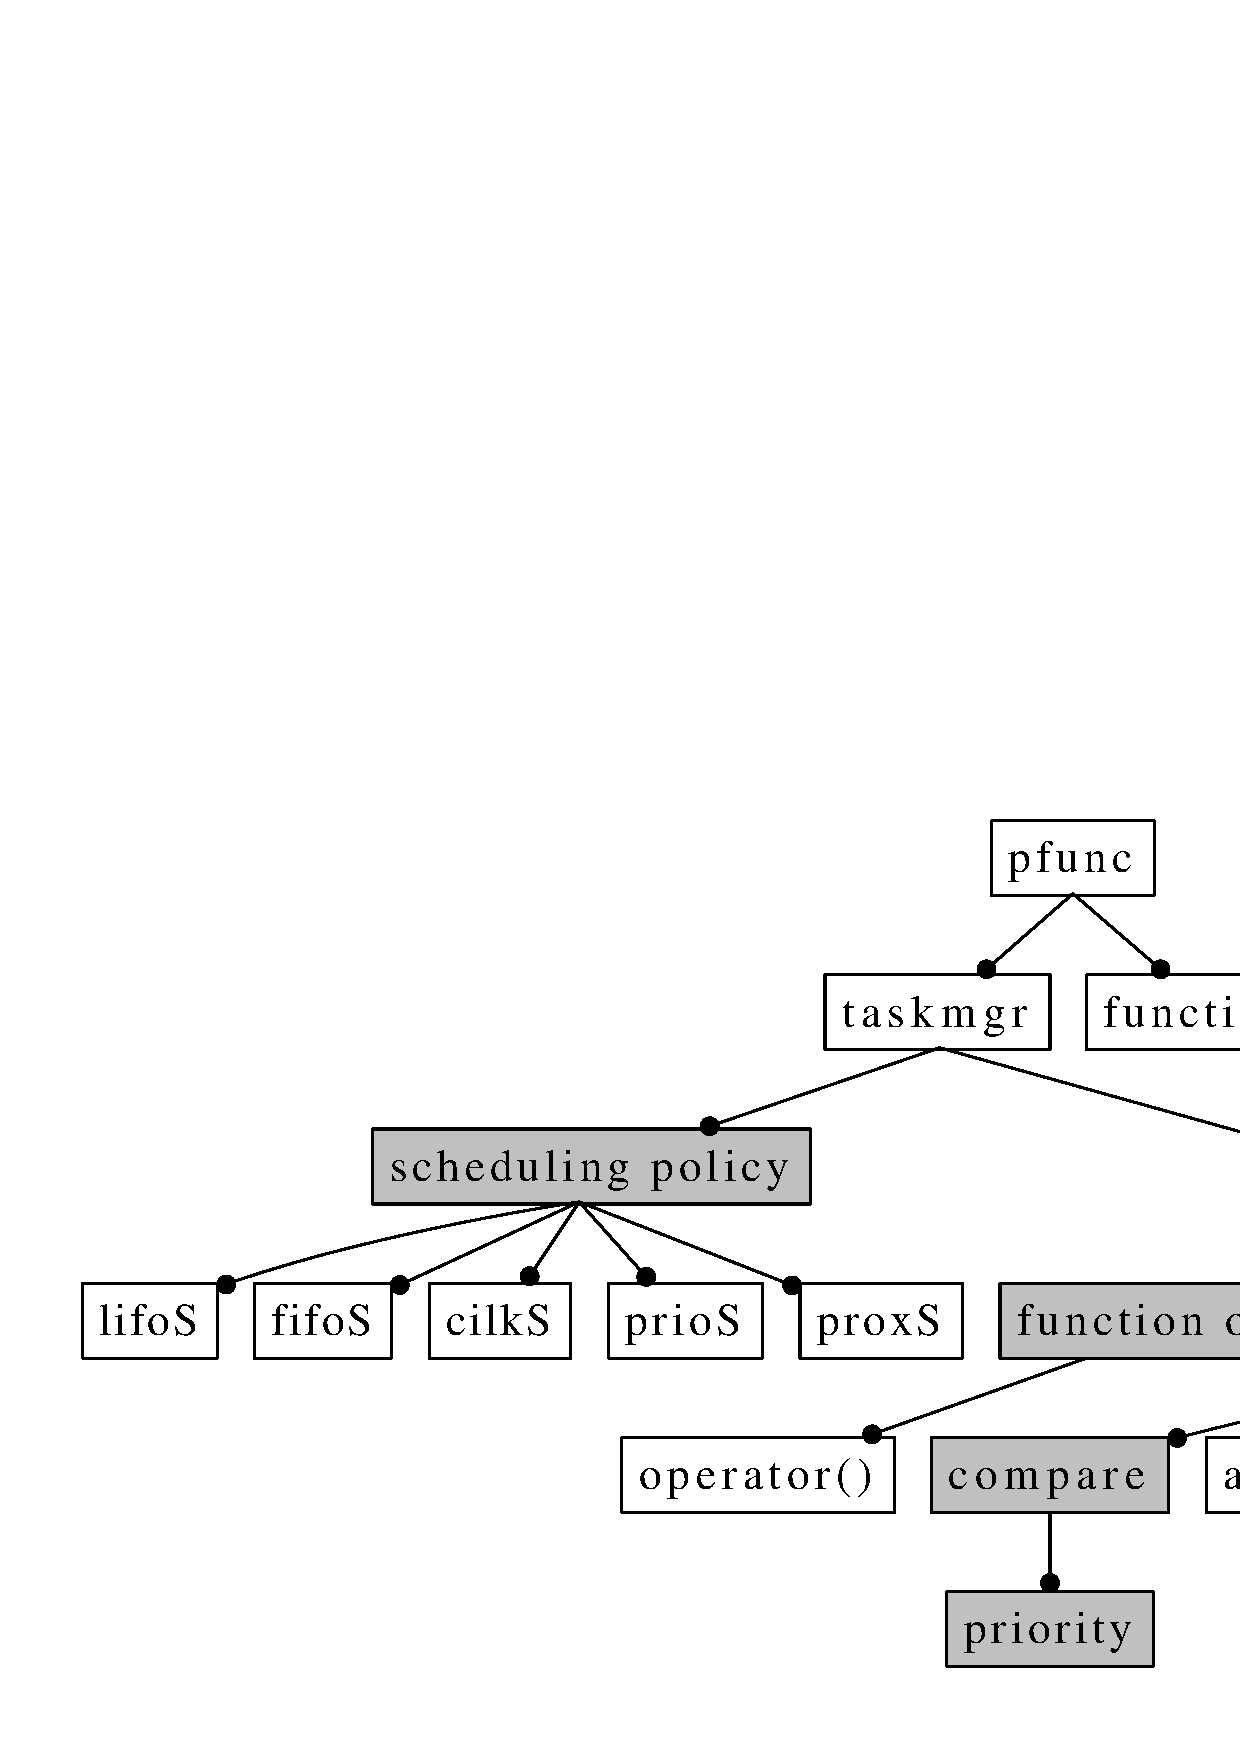
\includegraphics[width=0.90\textwidth]{figs/pfunc}
\caption{Feature diagram of the PFunc library showing the various features.
The features colored grey (scheduling policy, function object, compare and
priority) are generated based on user input.}
\label{fig:pfunc}
\end{figure}

As mentioned in Section~\ref{sec:introduction}, PFunc offers a wide variety
customizations to its users without incurring any runtime penalties. The first
step in using PFunc is to generate a customized library instance description
that best suits their needs (\Cpp{} only).  Then, the generated library
instance description is used to parallelize user applications. A feature
diagram of PFunc is shown in Figure~\ref{fig:pfunc}. The shaded blocks
represent features that can be customized and are described below.

\begin{list}{\labelitemi}{\leftmargin=1em}
% Scheduling policy
\item \textbf{Scheduling policy:}
The value provided to this feature determines the scheduling policy that is
used in the generated library instance description.  Figure~\ref{fig:pfunc}
enumerates all the built-in values that can be provided for this feature.
PFunc's users can also define custom scheduling polices and use them as the
value of this feature at instance generation time.
% Compare
\item \textbf{Compare:}
This feature represents the ordering function for task priorities and is used
only if the chosen scheduling policy requires task priorities (eg.,
\code{prioS}).  PFunc also allows customization of the \textbf{priority}
feature as it is inherited from the \textbf{compare} feature.
% Functor
\item \textbf{Function object:}
This feature allows users to specify the type of the function object that is
executed by the tasks.  By allowing the type of the function object to be
specified as a feature, PFunc successfully avoids paying the cost of virtual
function calls in the spawned tasks.~\footnote{This is true only when there is 
one function object that needs to be parallelized. In general, virtual function
call cannot be avoided if more than one type of function objects needs to be 
parallelized.} This is unlike other library-based approaches such as Intel's
Threading Building Blocks, where spawning a new task involves a virtual
function call.  
\end{list}

\subsection{\Cpp{}}
\label{sec:cxx:gen}
In \Cpp{}, the required library instance description can be generated using
template parameters to PFunc's \code{generator} interface. For example,
consider the following piece of code:

\begin{center}
\begin{minipage}{0.75\textwidth}
\begin{lstlisting}
typedef pfunc::generator<cilkS, /* scheduling policy */
                         pfunc::use_default, /* compare */
                         pfunc::use_default> my_pfunc; /*function object*/
\end{lstlisting}
\end{minipage}
\end{center}

\begin{figure}
\begin{center}
\begin{tabular}{|c|c|}
\hline
Feature & Default \\
\hline
\textbf{Scheduling policy} & \code{cilkS} \\
\hline
\textbf{Compare} & \func{std::less<int>} \\
\hline 
\textbf{Function object} & \code{struct \{ virtual void operator()() = 0; \};} \\
\hline
\end{tabular}
\end{center}
\caption{Default values for features.}
\label{fig:default}
\end{figure}

Here, we have generated an new library instance description of PFunc by
choosing the Cilk-style scheduling policy. The values for the \textbf{compare}
and \textbf{function object} features are allowed to be defaults. It is
possible to use \code{pfunc::use_default} for all the features
(Figure~\ref{fig:default}).  PFunc automatically chooses sensible values for the
features in this case.  The type \code{my\_pfunc} thus generated in our example
is a custom instance that can be used to parallelize user applications. In
PFunc, there are four important types that users are exposed to.  These are:
\code{attribute}, \code{group}, \code{task} and \code{taskmgr}.  Once the
required library instance description has been generated, these types can be
accessed as follows:

\begin{center}
\begin{minipage}{0.4\textwidth}
\begin{lstlisting}
my_pfunc::attribute attribute; 
my_pfunc::group group; 
my_pfunc::task task; 
my_pfunc::taskmgr taskmgr; 
\end{lstlisting}
\end{minipage}
\end{center}

% attribute
Objects of type \code{attribute} allow users to control the execution of
spawned tasks by setting attributes such as task priority and task affinity
(see Section~\ref{sec:attribute}).
% group
Objects of type \code{group} can be used to create collaborations of tasks that
can communicate with each other using point-to-point message passing and
barrier synchronization (see Section~\ref{sec:group}).
% task
Objects of type \code{task} are used as references to spawned tasks, which 
can be passed to other tasks. The ability to pass task references is crucial
for the support of multiple task completion notifications (see
Section~\ref{sec:spawn}).
% taskmgr
Finally, objects of type \code{taskmgr} manage threads and their task
queues, and are responsible for task scheduling (see Section~\ref{sec:spawn}).

\subsection{C}
In C, both because of the lack of support for generic programming and the
pitfalls of over-using preprocessor macros, PFunc pre-generates the library
instance descriptions for the users. The users are merely required
to then select the right library instance description from the avaible set of 
pre-generated descriptions. The currently available library instance
descriptions for C programmers are:

\begin{center}
\begin{tabular}{|c|c|c|c|}
\hline
Instance description & Scheduling policy & Compare, priority & Function type \\
\hline
\code{pfunc_cilk_*} & Cilk-style & \textbf{unused} & \code{void (*)(void*)} \\
\hline
\code{pfunc_lifo_*} & Queue & \textbf{unused} & \code{void (*)(void*)} \\
\hline
\code{pfunc_fifo_*} & Stack & \textbf{unused} & \code{void (*)(void*)} \\
\hline
\code{pfunc_prio_*} & Priority-based & \code{<} op, \code{int} & \code{void (*)(void*)} \\
\hline
\end{tabular}
\end{center}

The above table describes the four library instance descriptions that are
available to the C programmers.  Like in \Cpp{}, there are four important
types: \code{attribute}, \code{group}, \code{task} and \code{taskmgr}, which
are exposed to the users.  For example, consider the Cilk-style library
instance description.  The names by which these types can be accessed for the
Cilk-style instance description are \code{pfunc_cilk_attr_t},
\code{pfunc_cilk_group_t}, \code{pfunc_cilk_task_t} and
\code{pfunc_cilk_taskmgr_t}. 

\paragraph{Caveat} As PFunc is implemented completely in \Cpp{}, the C types
(\code{attribute, group, task, taskmgr}) are mere typed pointers to their
\Cpp{} counterparts. Consequently, before using these types (eg.,
\code{pfunc_cilk_attr_t}, \code{pfunc_cilk_group_t}, \code{pfunc_cilk_task_t}
and \code{pfunc_cilk_taskmgr_t}), they need to be initialized and cleared
explicility using calls to their respective \func{init} and \func{clear}
functions. This notion of initializing and clearing PFunc's C types will be
reinforced throughout the C examples described in this tutorial.
